\documentclass{article}
% --- watermark (auto-inserted) ---
\usepackage{xcolor}
\usepackage{xfp}% \fpeval; in the kernel since 2022, harmless on older LaTeX
\usepackage{draftwatermark}
\newlength{\watermarkTextWidth}
\AddToHook{begindocument/end}{%
  \SetWatermarkText{\normalfont Generated by The Agentic Scientist}%
  \SetWatermarkFontSize{10pt}%
  \SetWatermarkLightness{0.85}%
  \settowidth{\watermarkTextWidth}{\normalfont\fontsize{10pt}{12pt}\selectfont Generated by The Agentic Scientist}%
  \edef\watermarkScale{\fpeval{0.8 * sqrt(\paperwidth**2 + \paperheight**2) / \watermarkTextWidth}}%
  \edef\watermarkAngle{\fpeval{atand(\paperheight/\paperwidth)}}%
  \SetWatermarkScale{\watermarkScale}%
  \SetWatermarkAngle{\watermarkAngle}%
}
% --- end watermark ---

\usepackage{iclr2026_conference,times}
\usepackage[T1]{fontenc}
\usepackage[utf8]{inputenc}
\usepackage{amsmath,amssymb,booktabs,graphicx,longtable,subcaption}
\usepackage{hyperref,url}
\title{Cap-Dependent Task Budgets for Leaderboard Promotion}
\newcommand{\budget}{B}
\newcommand{\tol}{\varepsilon}
\begin{document}
\maketitle

\begin{abstract}
Multitask leaderboards aggregate heterogeneous scores, creating incentives to improve selected benchmark tasks rather than broad capability. How much targeted investment is needed to reach the top, and does the answer depend on the aggregation rule? We study a static score-space model: investment selects tasks, each selected score receives a bounded fraction of its remaining headroom, and competitors remain fixed. We compare arithmetic mean, ordinary median, and pairwise Borda aggregation on public HELM MMLU and Open LLM score snapshots. Independently checked allocation bounds reveal cap-dependent reversals: for one HELM target, mean versus median budgets change from 9 versus 12 tasks at full headroom to 23 versus 12 at half headroom; an Open LLM target exhibits the same qualitative reversal. Some promotions become unattainable under the smaller cap. These results reject a cap-independent resistance ordering on the evaluated instances. They quantify conditional score-space vulnerability, not the training data, compute, or money needed to realize such changes.
% @evidence[[paper_data.json#/final_evaluation/evaluation_evidence/episodes/0/solution/cases/0/observations]]
% @evidence[[derived/original_records.json]]
\end{abstract}

\section{Introduction}
Public multitask benchmarks compress a model's performance profile into a leaderboard position. MMLU and BIG-Bench Hard exemplify evaluations with heterogeneous component tasks, while HELM emphasizes transparency and breadth of evaluation \citep{Hendrycks2020MMLU,Suzgun2022BBH,Liang2022HELM}. Once adoption and recognition depend on position, a developer may have an incentive to concentrate resources on a subset of benchmark tasks. A leaderboard's aggregation rule determines which score changes are rewarded. Evaluating that incentive requires specifying both the allowed changes and the meaning of investment.

We ask a deliberately conditional question: on a fixed public score table, what is the smallest task subset whose improvement would make a target model co-first? Investment is the number of selected tasks, not the amount of training data. Each selected coordinate receives a stipulated fraction of its remaining score headroom; every unselected coordinate and every competitor's coordinate stays fixed. This model separates a leaderboard's response to score changes from the unresolved question of how reliably training can produce those changes. It is an analysis of a possible response envelope, not evidence that a developer can realize the envelope.

A common intuition is that the median should resist concentrated improvements because isolated extreme scores need not affect its value. That intuition does not settle the relative cost of reaching the top. A mean rewards every increment, whereas a median depends on crossing order-statistic thresholds. Reducing the permitted increment can change which threshold crossings remain available without proportionally changing the median's task budget. Conversely, a low starting median can require many changes even when a mean responds cheaply. The relevant object is therefore a budget conditioned jointly on the target, aggregation rule, and response cap.

Our study makes three concrete contributions. It defines a common bounded intervention model for mean, median, and Borda; expresses scalar allocation through sorting or threshold certificates and Borda through rival-aware integer constraints; and reports paired budgets, unattainability, and matched comparator results on frozen public score tables. The central finding is not a universally preferable aggregation rule. The same-target mean--median ordering reverses when the cap changes in both evaluated settings. Reference bounds and explicit failure states make that conclusion auditable without interpreting a timeout as impossibility.

The study is intentionally narrower than a strategic training equilibrium. Competitors do not react, task costs are uniform, and no model is trained. These restrictions preserve an interpretable comparison but preclude claims about real resource expenditure, general capability, or a population-wide frequency of reversal. The full target panel, including targets already co-first under a different rule, is retained rather than filtering to favorable examples.

\begin{figure}[t]
\centering

\includegraphics[width=\textwidth]{figures/score_space_overview.png}
\caption{The score-space intervention model. A fixed public score table and target define the comparison. Selecting tasks raises only the target's selected coordinates to a specified headroom cap. Mean, ordinary median, and rival-aware Borda yield a minimum task budget or certified unattainability. The cap describes a hypothetical response, not a measured training effect.}
\label{fig:overview}
\end{figure}

\section{Related Work}
\paragraph{Evaluation design and incentives.}
The benchmark lottery shows that task selection can alter comparative conclusions \citep{Dehghani2021Lottery}. Here the task set stays fixed while the aggregation rule and permitted response change. HELM's multidimensional evaluation and the language-model evaluation harness motivate explicit task definitions and reproducible score processing \citep{Liang2022HELM,Gao2023Harness}; our computations use released scores rather than rerunning either evaluation system. Analyses of leaderboard incentives and selective evaluation provide complementary reasons not to equate rank with general capability \citep{Singh2025Illusion}. Strategic post-training has also been modeled as an interaction between a benchmark designer and competing developers \citep{Chen2026Strategic}. We instead hold rivals fixed and measure discrete promotion budgets, without estimating an equilibrium or latent quality.

\paragraph{Social choice and targeted changes.}
Treating tasks as voters connects model evaluation with social choice \citep{Lanctot2023SocialChoice,Brandt2016Handbook}; aggregating rankings is also a classical information-retrieval problem \citep{Dwork2001Rank}. Strategic preference reporting \citep{Gibbard1973Manipulation} and election bribery \citep{Faliszewski2009Bribery} establish useful distinctions between aggregation and manipulation. Our intervention changes only a target's numerical task coordinates, according to a fixed response cap. It cannot arbitrarily rewrite rankings or remove competitors. In particular, a Borda calculation must update rivals as the target overtakes them, rather than compare against frozen Borda totals.

\paragraph{Robustness and contamination.}
Classical robust estimation distinguishes local influence from resistance under a specified contamination model \citep{Huber1964Robust,Hampel1974Influence,Rousseeuw1984Median}. These distinctions caution against importing a slogan about median robustness into an adaptive, bounded, top-rank objective. Our coordinates are heterogeneous tasks, not independent observations of a common location parameter. Benchmark leakage and rephrased contamination can affect measured model performance \citep{Zhou2023Cheater,Yang2023Rephrased}, but those findings do not calibrate our headroom response. We neither identify contaminated models nor infer that task-specific data necessarily produces the score increments analyzed here. The contribution is an instance-level comparison under stated assumptions, not a claim of first priority over all work on strategic evaluation.

\section{Method}
\subsection{Problem setup and intervention model}
Let $X\in[0,1]^{n\times d}$ contain higher-is-better task scores, with target row $t$ and original target vector $x=X_t$. For a selected task set $S\subseteq\{1,\ldots,d\}$ and cap $\rho$, define
\begin{equation}
 u_j(\rho)=\operatorname{round}_{10}\!\left(x_j+\rho(1-x_j)\right),\qquad
 y_j(S,\rho)=\begin{cases}u_j(\rho),&j\in S,\\x_j,&j\notin S.\end{cases}
 \label{eq:response}
\end{equation}
The evaluated positive caps are $\rho=1$ and $\rho=1/2$. Input scores and endpoints are rounded to ten decimal places. A separate no-update control uses zero response. Task selection is the decision variable; the cap is an externally specified condition, not a fitted learning curve. Figure~\ref{fig:overview} summarizes this distinction.
% @evidence[[source_evidence/downstream/program/src/program.py#L260]]
% @evidence[[paper_data.json#/final_evaluation/evaluation_evidence/episodes]]

Write $A_r(i;X)$ for row $i$'s aggregate under rule $r$, and $X^{t\leftarrow y}$ for the modified table. Promotion means co-first within tolerance $\tol=10^{-10}$:
\begin{equation}
 A_r(t;X^{t\leftarrow y})\geq \max_{i\ne t} A_r(i;X^{t\leftarrow y})-\tol.
 \label{eq:success}
\end{equation}
We minimize the uniform investment
\begin{equation}
 \budget_r(t,\rho)=\min_S\{|S|:\text{Equation~\eqref{eq:success} holds}\},
 \qquad b_r(t,\rho)=\budget_r(t,\rho)/d.
 \label{eq:objective}
\end{equation}
If no subset succeeds, $\budget_r=\infty$. An empty successful subset has budget zero; an empty response reporting unattainability does not. Co-first is weaker than strict victory, and the results do not address arbitrary tie-breaking policies.
% @evidence[[source_evidence/downstream/program/src/program.py#L1]]

\subsection{Design rationale and compared approaches}
We compare arithmetic mean, ordinary median, and pairwise Borda on identical targets and endpoints. The even median averages the two central order statistics. Borda awards one point for a task-level pairwise win and half a point for a tie, then averages across opponents and tasks:
\begin{equation}
 A_{\mathrm{B}}(i;X)=\frac{1}{d(n-1)}\sum_{j=1}^{d}\sum_{h\ne i}
 \left[\mathbf{1}\{X_{ij}>X_{hj}\}+\tfrac12\mathbf{1}\{X_{ij}=X_{hj}\}\right].
 \label{eq:borda}
\end{equation}
Changing the target can lower a rival's Borda total even though the rival's underlying task scores are unchanged.
% @evidence[[source_evidence/downstream/program/src/program.py#L50]]

The hypothesis is conditional: the ordering of task budgets need not survive a change in cap. This follows mechanistically from distinct sufficient statistics. Mean uses total added score mass; median uses central threshold crossings; Borda uses pairwise crossings against the whole competitor population. None of these mechanisms implies the same ranking of investment costs on every target vector.

There is nevertheless a simple within-rule restriction. Holding the table and target fixed, a larger cap weakly expands the set of successful subsets. Thus, with infinity ordered above finite budgets,
\begin{equation}
 \rho_1\leq\rho_2\quad\Longrightarrow\quad
 \budget_r(t,\rho_1)\geq\budget_r(t,\rho_2).
 \label{eq:monotone}
\end{equation}
This implication follows from the same target--rival monotonicity used by the endpoint test. It does not order different rules: their budgets may increase by different amounts when the cap shrinks. Observing a reversal between rules therefore does not contradict monotonicity of either rule's own budget. This separation distinguishes the proposed comparison from an assertion that a smaller permitted improvement can make promotion cheaper.
% @evidence[[source_evidence/downstream/program/src/program.py#L260]]
% @evidence[[source_evidence/downstream/program/src/program.py#L193]]

Allocation methods are compared with no intervention, marginal greedy selection, and a seeded random task order evaluated by successive prefixes. Marginal greedy chooses the task producing the largest current improvement in the target's gap to its strongest rival, with deterministic task-order ties. A random order is drawn for each decision, not optimized over many orders. These are selection policies under the same response model, not alternative training procedures. The original development comparator uses exhaustive allocation on small tables and greedy allocation otherwise; its selection score does not supply a matched final population comparison.
% @evidence[[source_evidence/downstream/baseline/src/program.py#L59]]
% @evidence[[data/protocol.json#/baselines]]
% @evidence[[paper_data.json#/downstream_study]]

\subsection{Scalar allocation certificates}
For mean and median, competitors' aggregates stay fixed. Let $c_r=\max_{i\ne t}A_r(i;X)$. Raising selected coordinates to their endpoints cannot reduce any studied aggregate or worsen any target--rival gap. Thus the all-task endpoint vector certifies reachability: if it cannot win, no subset can. Conversely, because selected tasks have unit cost and no penalty for a larger allowed response, endpoint updates suffice for the stated optimization problem.

For the mean, let $g_j=u_j-x_j$, and sort gains decreasingly as $g_{(1)}\geq\cdots\geq g_{(d)}$. The minimum finite budget is the smallest $k$ satisfying
\begin{equation}
 \sum_{\ell=1}^{k} g_{(\ell)}\geq d\bigl(c_{\mathrm{mean}}-\tol-\bar{x}\bigr).
 \label{eq:mean}
\end{equation}
No other $k$ tasks can supply more gain, giving a cardinality certificate rather than just a successful witness.
% @evidence[[source_evidence/downstream/program/src/program.py#L73]]

For odd $d=2m+1$, median success requires at least $m+1$ coordinates at or above $c_{\mathrm{median}}-\tol$. Count those already above that threshold, then count coordinates whose endpoint crosses it. The required number of crossings gives the minimum if enough are available. For even $d=2m$, success depends on the sum of the two central values, not a single threshold. The solver enumerates candidate lower central endpoints and the smallest compatible upper endpoint. It checks the nested requirements of at least $m+1$ values above the lower endpoint and at least $m$ above the upper endpoint, sharing upgrades where possible. Final aggregate checks protect the numerical boundary. The small even-dimensional setting also uses exhaustive subset verification. Appendix~\ref{sec:scalar} gives the counting construction.
% @evidence[[source_evidence/downstream/program/src/program.py#L82]]
% @evidence[[source_evidence/downstream/program/src/program.py#L93]]
% @evidence[[source_evidence/downstream/program/src/program.py#L129]]

\subsection{Rival-aware Borda allocation}
Use twice-credit integer totals $T_i=2d(n-1)A_{\mathrm{B}}(i;X)$. Let $\delta_{ij}\in\{0,1,2\}$ be the increase in the target's twice-credit against rival $i$ on task $j$, and $G_j=\sum_{i\ne t}\delta_{ij}$. Selecting task $j$ increases the target's total by $G_j$ and decreases rival $i$'s total by $\delta_{ij}$. With binary task indicators $z_j$, the necessary and sufficient constraints are
\begin{equation}
 \sum_j (G_j+\delta_{ij})z_j\geq D_i,
 \quad D_i=\left\lceil T_i-T_t-2d(n-1)\tol\right\rceil,
 \quad i\ne t.
 \label{eq:cover}
\end{equation}
Only initially positive deficits constrain the solution, since all gap improvements are nonnegative. This formulation accounts for changing rival totals explicitly.
% @evidence[[source_evidence/downstream/program/src/program.py#L193]]

The supplied selected source builds a feasible gain-ordered prefix, deletes unnecessary tasks, and searches smaller cardinalities using individual-rival bounds and suffix pruning. Search is bounded by a deadline and a node limit; on interruption it returns a verified incumbent, not an optimality assertion. In the recorded original instances, independent reference bounds close and match every finite returned cardinality. That observed agreement is stronger than a feasible-witness check, but it does not establish exactness for arbitrary larger instances or superiority of a particular search component. No controlled component ablation is available.
% @evidence[[source_evidence/downstream/program/src/program.py#L160]]
% @evidence[[paper_data.json#/final_evaluation/evaluation_evidence/episodes]]

\section{Public Score Tables and Comparison Protocol}
\paragraph{Snapshots and preprocessing.}
The study uses HELM's MMLU release v1.13.0 and the pinned Open LLM contents snapshot, acquired on 7 November 2026. HELM contributes 57 subject scores; Open LLM contributes six normalized leaderboard columns: IFEval, BBH, MATH Lvl 5, GPQA, MuSR, and MMLU-PRO. Open LLM scores are divided by 100; its additional raw columns are not treated as independent tasks. The comparison recomputes all three aggregation rules from these component scores. It is not a claim about the live ordering displayed by either website.
% @evidence[[data/helm.json#/tasks]]
% @evidence[[data/openllm.json#/tasks]]
% @evidence[[data/protocol.json#/normalization]]
% @evidence[[paper_data.json#/final_evaluation/evaluation_evidence/episodes]]

Score content and known model aliases are clustered before a deterministic content-based split separates development from final analysis. Exact duplicates are collapsed; normalization is applied after assignment. The frozen final competitor tables, not just the selected targets, determine every comparison. Known alias matching reduces exact overlap but cannot establish unseen-model-family independence because lineage information is incomplete. Appendix~\ref{sec:repro} specifies versions, hashes, and the acquisition code.

\paragraph{Targets and matched comparisons.}
Each final score table has eight fixed targets, selected at rank-spaced positions among nonwinners under its original arithmetic mean. Target selection is not repeated separately for each rule. Consequently, a target can already be co-first under median or Borda. We retain such zero-budget cases. Each target is assessed under every rule at both positive caps, keeping all other inputs fixed. Target labels are frozen row indices, not model-family categories.
% @evidence[[data/protocol.json#/target_selection]]
% @evidence[[derived/summary.json#/targets]]

The records contain three seeded executions, with seeds 42011, 42013, and 42017, of the same target instances. There are 48 distinct target--rule--cap decisions per score table. Independent validation recomputes aggregate success and checks the reference bounds. The reference uses exhaustive subsets for the six-task table, sorting or threshold counting for scalar rules on HELM, and a time-limited binary optimization reference for HELM Borda. We report a finite optimum only where a valid witness and matching lower and upper bounds are recorded; unresolved optimization would remain a bound interval. Independently certified unattainability is kept separate from missing or failed computation.
% @evidence[[paper_data.json#/final_evaluation/evaluation_evidence/episodes]]
% @evidence[[data/protocol.json#/baselines]]

\paragraph{Checks and uncertainty.}
Task permutations, constant-score tables, and zero-update controls test implementation behavior and are excluded from the empirical target denominator. A recorded reset replay checks a repeated status/effort signature. Repeated seeds do not resample tasks or models. We therefore report deterministic paired differences and observed repeatability, not confidence intervals for an unspecified population. The random comparator's range reflects only its recorded orders. No statistical test is used to turn these fixed-panel counterexamples into a universal rule ranking.

\section{Results: Cap-Dependent Promotion Budgets}
\subsection{Within-target reversals}
Table~\ref{tab:budgets} reports every original target. Figure~\ref{fig:paired} places the mean and median budgets on common normalized axes. Points above the diagonal require more tasks under median; points below it require more under mean. The shaded rails retain unattainable cases rather than assigning them an artificial large finite budget. Multiplicities are explicit, and seeded repeats are not plotted as independent targets.

For HELM target 10, the mean/median budgets are 9/12 tasks at full headroom and 23/12 at half headroom. For Open LLM target 1609, they are 2/3 and 4/3, respectively. Thus the direction of the same-target comparison reverses in both score tables. These examples refute a cap-independent ordering on these instances; they do not estimate how frequently such reversals occur among future models.
% @evidence[[paper_data.json#/final_evaluation/evaluation_evidence/episodes/0/solution/cases/0/observations]]
% @evidence[[paper_data.json#/final_evaluation/evaluation_evidence/episodes/0/solution/cases/4/observations]]

The reversal is interpretable without attributing it to training. Smaller increments reduce the total gain available to the mean, requiring additional coordinates. The median can retain its task count when the necessary endpoint threshold crossings remain possible. HELM targets 37, 18, and 28 exhibit unchanged median counts across the two caps while their mean counts increase. This is a property of their observed score geometry under the stipulated response, not a claim that median is insensitive to cap changes in general. HELM target 40 already has median budget zero at both caps despite being a mean-selected nonwinner.
% @evidence[[derived/original_records.json]]

\begin{table}[t]
\centering\small
\caption{Minimum selected-task counts on all original targets. $\infty$ means unattainable under the stated cap. Every finite count matches a closed independent reference bound in each recorded seeded execution. Task counts are within-snapshot investments, not calibrated training costs.}
\label{tab:budgets}
\begin{tabular}{llrrrrrr}
\toprule
 & & \multicolumn{3}{c}{$\rho=1$} & \multicolumn{3}{c}{$\rho=1/2$} \\
Snapshot & Target & Mean & Median & Borda & Mean & Median & Borda \\
\midrule
HELM MMLU & 40 & 1 & 0 & 4 & 1 & 0 & 4 \\
 & 10 & 9 & 12 & 34 & 23 & 12 & 39 \\
 & 37 & 12 & 16 & 41 & 36 & 16 & 50 \\
 & 18 & 13 & 18 & 41 & 40 & 18 & 52 \\
 & 28 & 16 & 21 & 46 & 49 & 21 & $\infty$ \\
 & 16 & 21 & 24 & 50 & $\infty$ & $\infty$ & $\infty$ \\
 & 26 & 25 & 29 & 51 & $\infty$ & $\infty$ & $\infty$ \\
 & 20 & 46 & 29 & 53 & $\infty$ & $\infty$ & $\infty$ \\
\midrule
Open LLM & 803 & 1 & 1 & 1 & 1 & 1 & 1 \\
 & 1188 & 2 & 2 & 5 & 3 & 3 & 5 \\
 & 1609 & 2 & 3 & 5 & 4 & 3 & 5 \\
 & 1566 & 2 & 3 & 6 & 4 & 4 & $\infty$ \\
 & 1101 & 2 & 3 & 6 & 5 & 4 & $\infty$ \\
 & 365 & 3 & 3 & 6 & 5 & 4 & $\infty$ \\
 & 1331 & 3 & 3 & 6 & 6 & $\infty$ & $\infty$ \\
 & 1870 & 4 & 4 & 6 & $\infty$ & $\infty$ & $\infty$ \\
\bottomrule
\end{tabular}
% @evidence[[paper_data.json#/final_evaluation/evaluation_evidence/episodes]]

\end{table}

\begin{figure}[t]
\centering
\begin{subfigure}{\textwidth}
\centering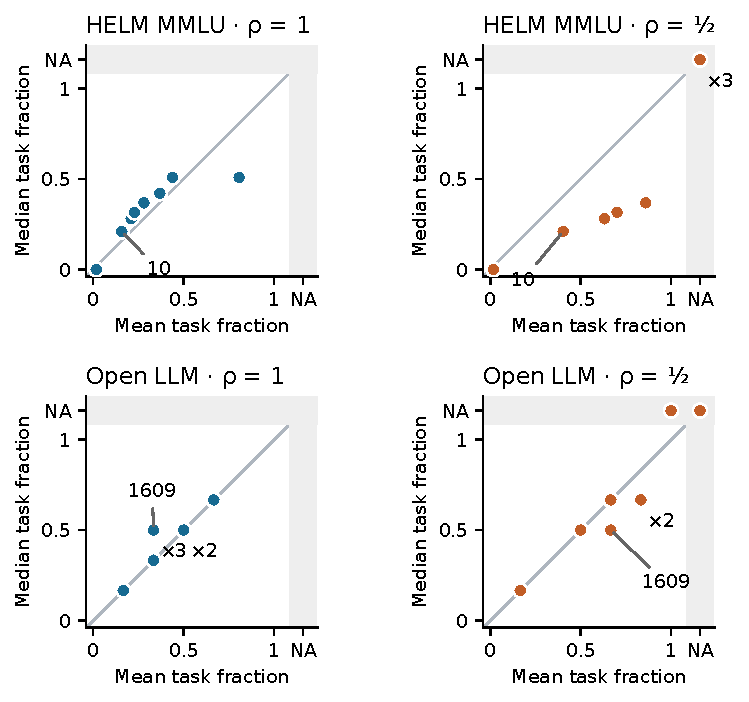
\includegraphics[width=\textwidth]{figures/paired_mean_median_budgets.pdf}
\end{subfigure}
\caption{Paired minimum task fractions for identical targets. Top: HELM; bottom: Open LLM. Left: full headroom; right: half headroom. NA rails indicate certified unattainability, not missing values or an additional numeric range. Annotated row indices identify targets that reverse their mean--median ordering. Labels $\times k$ denote coincident target points. All finite points have matching independent lower and upper cardinality bounds.}
\label{fig:paired}
% @evidence[[derived/original_records.json]]
\end{figure}

\subsection{Reachability and Borda}
At full headroom, all eight targets in each table are reachable under all three rules. This is expected structurally: selecting every coordinate sets the target to the scale maximum. The informative full-headroom quantity is therefore the minimum task budget, not reachability alone. At half headroom, HELM has five reachable targets under mean, five under median, and four under Borda; Open LLM has seven, six, and three. Figure~\ref{fig:reachability} uses the same target denominator throughout. An all-task cap that fails the rank condition certifies these unattainable cases. Such a result is a limit of the intervention model, not evidence of an unsuccessful training run or a solver timeout.
% @evidence[[derived/summary.json#/reachability]]

Borda can require a large selected subset because improving a task matters through the rival crossings it enables. For Open LLM target 1566, full-headroom Borda requires all six tasks, but half-headroom Borda is unattainable; mean and median remain reachable with four tasks at half headroom. HELM target 28 is also unreachable under half-headroom Borda while mean and median remain reachable. These are comparisons between precisely defined rule-and-cap configurations. They do not isolate a causal benefit of ordinal aggregation, since the aggregation objective itself changes.
% @evidence[[derived/original_records.json]]

\begin{figure}[t]
\centering
\begin{subfigure}{\textwidth}
\centering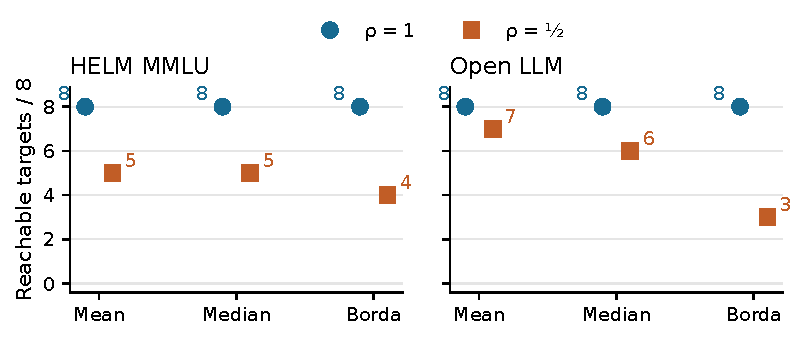
\includegraphics[width=\textwidth]{figures/cap_conditioned_reachability.pdf}
\end{subfigure}
\caption{Reachable original targets out of eight, by aggregation rule and response cap. The denominator excludes seeded repeats and synthetic controls. Reachability means co-first under the cap, not general model improvement. All full-headroom cases are reachable; half-headroom failures differ by rule and score table.}
\label{fig:reachability}
% @evidence[[derived/summary.json#/reachability]]
\end{figure}

\subsection{Allocation checks and comparator interpretation}
Across the original decisions, all recorded reference intervals close. Every finite selected cardinality equals its reference minimum, and every reported unattainable decision agrees with the independent reference. The selected task subsets are identical across the three seeds, not merely equal in size. These observations support the precision of the reported finite-instance comparisons, not a claim about unrestricted solver completeness.
% @evidence[[derived/summary.json]]

Marginal greedy matches the minimum on the recorded feasible mean and Borda decisions. It can miss median budgets because immediate marginal changes do not necessarily reward the threshold crossings needed for eventual promotion. For HELM target 28 at half headroom, the certified median minimum is 21 tasks, compared with 52 for the recorded greedy policy. This gap concerns a selection policy on that instance; no ablation identifies which internal solver component accounts for it. Nor is it a general advantage over the original development comparator: the frozen selection had no aggregate development-score improvement over that comparator. Matched random-order costs and all selected subsets are supplied in the supplement and machine-readable records.
% @evidence[[derived/summary.json#/comparators]]
% @evidence[[derived/original_records.json]]
% @evidence[[paper_data.json#/downstream_study/search_score_delta]]

\section{Discussion and Limitations}
\paragraph{What the investment measures.}
A task count measures concentration of intervention support. It does not measure examples, tokens, training steps, compute, or money. The response in Equation~\eqref{eq:response} is hypothetical and favorable: all selected improvements are jointly available, improvements do not spill into unselected tasks, and no forgetting occurs. Real training can violate every condition. A smaller task budget can therefore coexist with a larger real training cost. The empirical conclusions apply only to the stated score response, uniform task costs, and fixed competitors.

\paragraph{Why rule robustness is conditional.}
Median robustness in a location-estimation problem does not by itself determine the cost of overtaking a particular competitor. Here the objective is relative rank, and the target's starting position matters. Borda additionally depends on the whole competitor population; mean and median depend on their respective strongest rival aggregate. A change in the competitor set or task composition could change the comparisons. The analysis holds those objects fixed, rather than selecting a favorable population for each rule. Normalizing by task count enables a visual comparison but does not make selecting a subject equivalent in practical effort to selecting an entire benchmark.

\paragraph{Coverage and uncertainty.}
The paired design identifies cap sensitivity on the observed instances, not how common the phenomenon is beyond them. Targets are mean-rank stratified rather than a random model sample. The two score snapshots share an evaluation ecosystem and can include related model lineages. Hash and alias separation does not establish independence of model development or broad transfer. Only two positive caps were evaluated; the figures are discrete comparisons, not continuous response frontiers. No composition resampling, strict-victory sensitivity, heterogeneous-cost study, or empirical training-response calibration is available. These omissions constrain generalization but do not invalidate the displayed within-target counterexamples.
% @evidence[[derived/summary.json]]

\paragraph{Computation and scientific scope.}
A feasible witness alone would not certify a minimum; a time limit alone would not certify impossibility. We preserve both distinctions. Bound closure happens to support exact cardinalities on the recorded original instances, although Borda search is bounded in the implementation. The separate final assessment is completed and qualified; that status neither establishes novelty nor enlarges the scope of the scientific conclusions. The development comparison has no positive aggregate difference, and no component ablation supports a claim of optimizer superiority. Public availability of score files also does not settle their redistribution rights; the reproduction instructions preserve upstream provenance and describe reacquisition rather than assuming a code or model license covers score data.
% @evidence[[paper_data.json#/final_evaluation/status]]
% @evidence[[paper_data.json#/final_evaluation/outcome]]
% @evidence[[paper_data.json#/downstream_study/search_score_delta]]

\section{Conclusion}
Targeted leaderboard promotion has no meaningful task budget until both the aggregation rule and the allowed score response are specified. Under a bounded headroom model on two frozen public score tables, paired minimum budgets reverse their mean--median ordering for some targets when the cap is reduced. Reachability also changes by rule, including cases where using every task is insufficient. The evidence supports these finite-instance, conditional conclusions rather than a universal ranking of aggregation rules.

The practical implication is methodological: report the target score vector, response assumptions, competitor population, success criterion, and allocation bounds together. A single aggregate vulnerability score hides distinctions between inexpensive promotion, already being co-first, and promotion that is impossible under the cap. Extending this analysis to real resource allocation requires evidence linking training investments to joint score changes and their side effects. Until such calibration is available, task-count budgets are interpretable counterfactual diagnostics, not estimates of the cost of producing a better model.

\clearpage
\bibliography{references}
\bibliographystyle{iclr2026_conference}
\clearpage
\appendix
\section{Supplementary Information}

\subsection{Endpoint reduction and scalar certificates}\label{sec:scalar}
For each rule, increasing only a target coordinate weakly improves every target--rival gap. For mean and median this follows from coordinatewise monotonicity with unchanged rival aggregates. For Borda, the target gains pairwise credit while any overtaken rival loses the corresponding credit. Consequently, if the all-task endpoint vector is unsuccessful, every subset is unsuccessful. If a selected task could instead receive any intermediate increase below its endpoint at the same unit cost, replacing it by its endpoint cannot destroy success. This endpoint reduction does not apply when improvements incur magnitude-dependent costs, adversely affect other coordinates, or provoke responding rivals.

For mean, the largest-gain prefix maximizes added score over subsets of a fixed size, proving Equation~\eqref{eq:mean}. For odd median, put $h=c_{\mathrm{median}}-\tol$, $a=\#\{j:x_j\geq h\}$, and $p=\#\{j:x_j<h\leq u_j\}$. With $d=2m+1$, the finite minimum is $k=\max(0,m+1-a)$ if $k\leq p$, and is otherwise unattainable. This is a threshold count, not a local derivative of the median.
% @evidence[[source_evidence/downstream/program/src/program.py#L73]]
% @evidence[[source_evidence/downstream/program/src/program.py#L82]]

For the even median, let $d=2m$ and let $\mathcal{E}=\{x_j,u_j:j=1,\ldots,d\}$ be the set of endpoints. Enumerate $\ell\in\mathcal{E}$ and choose the smallest $h\in\mathcal{E}$ with $h\geq\ell$ and $(\ell+h)/2\geq c_{\mathrm{median}}-\tol$. At least $m+1$ coordinates must be at least $\ell$, and at least $m$ must be at least $h$. Set
\[
 a_\ell=\max(0,m+1-\#\{x_j\geq\ell\}),\qquad
 a_h=\max(0,m-\#\{x_j\geq h\}).
\]
Partition available upgrades into shared crossings $x_j<\ell,\ u_j\geq h$, lower-only crossings $x_j<\ell\leq u_j<h$, and upper-only crossings $\ell\leq x_j<h\leq u_j$. Shared crossings cover both deficits; the other two types cover one each. If either deficit exceeds its total available crossings, discard the endpoint pair. Otherwise use shared crossings up to the larger deficit and fill remaining deficits from their dedicated types. Checking the resulting median and taking the smallest cardinality over endpoints yields the implemented construction. For a fixed lower endpoint, increasing the upper threshold only shrinks feasible choices, so the smallest compatible upper endpoint suffices. On the six-task table, exhaustive verification also checks scalar cardinalities. These are explanations of the inspected implementation, not additional experimental findings.
% @evidence[[source_evidence/downstream/program/src/program.py#L93]]
% @evidence[[source_evidence/downstream/program/src/program.py#L129]]

\subsection{Borda constraints and bounded search}
Equation~\eqref{eq:cover} follows by subtracting the updated rival total $T_i-\sum_j\delta_{ij}z_j$ from the updated target total $T_t+\sum_jG_jz_j$. Integer ceiling converts the aggregate tolerance to a gap constraint. Every coefficient is nonnegative, so initially nonthreatening rivals stay nonthreatening. Full-cap failure of any constraint certifies unattainability. A feasible subset is always checked against the complete active-rival constraints, not just the reduced search system.

Let $D=\max_iD_i$ and let $U$ be the current feasible cardinality. For a subset with at most $U$ tasks, the rival-specific contribution is bounded by $2U$. Satisfying the largest deficit therefore requires common gain at least $D-2U$. Rivals with deficit at most that value can safely be omitted during improvement search. Zero-common-gain tasks do not help. Independent-rival sorted coefficient sums give lower cardinality bounds. Branch search prunes a node if the largest remaining coefficients for any rival cannot cover its residual deficit within the remaining task slots. Its node limit is 20,000; the solver uses 90\% of the supplied work allowance and divides remaining time among pending Borda decisions. These are source settings, not measured speedups.
% @evidence[[source_evidence/downstream/program/src/program.py#L160]]
% @evidence[[source_evidence/downstream/program/src/program.py#L193]]
% @evidence[[source_evidence/downstream/program/src/program.py#L268]]

There is no assertion of a generic greedy approximation guarantee: guarantees for submodular maximization require specific objective and constraint assumptions \citep{Nemhauser1978Submodular}. Nor is this a robust optimization problem that optimizes against a calibrated uncertainty set. Robust optimization provides a different treatment of uncertain coefficients and conservatism \citep{BenTal1998Robust,Bertsimas2004Price,Bertsimas2011Theory}. Our response cap is fixed for each conditional comparison. It is not a distributional estimate, a worst-case set learned from interventions, or a guarantee about actual score changes.

\subsection{Complete allocation and comparator tables}
Tables below contain all original target--rule--cap combinations. Selected minima and their task subsets repeat across the recorded seeds. Greedy counts are unchanged across these seeds; random-prefix counts can differ, so their range is shown rather than treating the best order as the policy. Normalized counts are rounded for display only. The CSV retains full task indices, exact source pointers, seed-level comparator counts, and the recorded reference bounds. For unattainability, the underlying reference uses an out-of-range cardinality sentinel; the tables display $\infty$ instead of that sentinel. No sentinel is interpreted as measured investment.
% @evidence[[derived/allocations.csv]]
\begingroup\small
\begin{longtable}{llrrr rr r rr}
\caption{Complete original decisions for HELM MMLU. $B$ is the selected minimum; $L=U$ is the independent reference bound when finite. $G$ is marginal greedy; $R$ is the range across the recorded seeded random orders. $\infty$ denotes independently certified unattainability, not zero investment.}\\
\toprule
Target & Rule & $\rho$ & $B$ & $B/d$ & $L$ & $U$ & $G$ & \multicolumn{2}{c}{$R$ (min--max)} \\
\midrule\endfirsthead
\toprule Target & Rule & $\rho$ & $B$ & $B/d$ & $L$ & $U$ & $G$ & \multicolumn{2}{c}{$R$ (min--max)} \\ \midrule\endhead
40 & Mean & 1.0 & 1 & 0.018 & 1 & 1 & 1 & 1 & 1 \\
40 & Mean & 0.5 & 1 & 0.018 & 1 & 1 & 1 & 1 & 1 \\
40 & Median & 1.0 & 0 & 0.000 & 0 & 0 & 0 & 0 & 0 \\
40 & Median & 0.5 & 0 & 0.000 & 0 & 0 & 0 & 0 & 0 \\
40 & Borda & 1.0 & 4 & 0.070 & 4 & 4 & 4 & 15 & 23 \\
40 & Borda & 0.5 & 4 & 0.070 & 4 & 4 & 4 & 12 & 17 \\
10 & Mean & 1.0 & 9 & 0.158 & 9 & 9 & 9 & 16 & 23 \\
10 & Mean & 0.5 & 23 & 0.404 & 23 & 23 & 23 & 38 & 38 \\
10 & Median & 1.0 & 12 & 0.211 & 12 & 12 & 12 & 16 & 18 \\
10 & Median & 0.5 & 12 & 0.211 & 12 & 12 & 16 & 20 & 32 \\
10 & Borda & 1.0 & 34 & 0.596 & 34 & 34 & 34 & 41 & 47 \\
10 & Borda & 0.5 & 39 & 0.684 & 39 & 39 & 39 & 46 & 50 \\
37 & Mean & 1.0 & 12 & 0.211 & 12 & 12 & 12 & 22 & 27 \\
37 & Mean & 0.5 & 36 & 0.632 & 36 & 36 & 36 & 47 & 49 \\
37 & Median & 1.0 & 16 & 0.281 & 16 & 16 & 16 & 19 & 22 \\
37 & Median & 0.5 & 16 & 0.281 & 16 & 16 & 22 & 47 & 50 \\
37 & Borda & 1.0 & 41 & 0.719 & 41 & 41 & 41 & 46 & 48 \\
37 & Borda & 0.5 & 50 & 0.877 & 50 & 50 & 50 & 53 & 54 \\
18 & Mean & 1.0 & 13 & 0.228 & 13 & 13 & 13 & 23 & 25 \\
18 & Mean & 0.5 & 40 & 0.702 & 40 & 40 & 40 & 50 & 51 \\
18 & Median & 1.0 & 18 & 0.316 & 18 & 18 & 18 & 20 & 25 \\
18 & Median & 0.5 & 18 & 0.316 & 18 & 18 & 29 & 39 & 42 \\
18 & Borda & 1.0 & 41 & 0.719 & 41 & 41 & 41 & 47 & 49 \\
18 & Borda & 0.5 & 52 & 0.912 & 52 & 52 & 52 & 55 & 55 \\
28 & Mean & 1.0 & 16 & 0.281 & 16 & 16 & 16 & 24 & 31 \\
28 & Mean & 0.5 & 49 & 0.860 & 49 & 49 & 49 & 54 & 55 \\
28 & Median & 1.0 & 21 & 0.368 & 21 & 21 & 21 & 24 & 25 \\
28 & Median & 0.5 & 21 & 0.368 & 21 & 21 & 52 & 54 & 57 \\
28 & Borda & 1.0 & 46 & 0.807 & 46 & 46 & 46 & 50 & 51 \\
28 & Borda & 0.5 & $\infty$ & $\infty$ & $\infty$ & $\infty$ & $\infty$ & $\infty$ & $\infty$ \\
16 & Mean & 1.0 & 21 & 0.368 & 21 & 21 & 21 & 29 & 32 \\
16 & Mean & 0.5 & $\infty$ & $\infty$ & $\infty$ & $\infty$ & $\infty$ & $\infty$ & $\infty$ \\
16 & Median & 1.0 & 24 & 0.421 & 24 & 24 & 24 & 25 & 28 \\
16 & Median & 0.5 & $\infty$ & $\infty$ & $\infty$ & $\infty$ & $\infty$ & $\infty$ & $\infty$ \\
16 & Borda & 1.0 & 50 & 0.877 & 50 & 50 & 50 & 52 & 52 \\
16 & Borda & 0.5 & $\infty$ & $\infty$ & $\infty$ & $\infty$ & $\infty$ & $\infty$ & $\infty$ \\
26 & Mean & 1.0 & 25 & 0.439 & 25 & 25 & 25 & 34 & 39 \\
26 & Mean & 0.5 & $\infty$ & $\infty$ & $\infty$ & $\infty$ & $\infty$ & $\infty$ & $\infty$ \\
26 & Median & 1.0 & 29 & 0.509 & 29 & 29 & 29 & 29 & 29 \\
26 & Median & 0.5 & $\infty$ & $\infty$ & $\infty$ & $\infty$ & $\infty$ & $\infty$ & $\infty$ \\
26 & Borda & 1.0 & 51 & 0.895 & 51 & 51 & 51 & 53 & 53 \\
26 & Borda & 0.5 & $\infty$ & $\infty$ & $\infty$ & $\infty$ & $\infty$ & $\infty$ & $\infty$ \\
20 & Mean & 1.0 & 46 & 0.807 & 46 & 46 & 46 & 47 & 47 \\
20 & Mean & 0.5 & $\infty$ & $\infty$ & $\infty$ & $\infty$ & $\infty$ & $\infty$ & $\infty$ \\
20 & Median & 1.0 & 29 & 0.509 & 29 & 29 & 29 & 29 & 29 \\
20 & Median & 0.5 & $\infty$ & $\infty$ & $\infty$ & $\infty$ & $\infty$ & $\infty$ & $\infty$ \\
20 & Borda & 1.0 & 53 & 0.930 & 53 & 53 & 53 & 53 & 54 \\
20 & Borda & 0.5 & $\infty$ & $\infty$ & $\infty$ & $\infty$ & $\infty$ & $\infty$ & $\infty$ \\
\bottomrule\end{longtable}
% @evidence[[paper_data.json#/final_evaluation/evaluation_evidence/episodes]]
\begin{longtable}{llrrr rr r rr}
\caption{Complete original decisions for Open LLM. $B$ is the selected minimum; $L=U$ is the independent reference bound when finite. $G$ is marginal greedy; $R$ is the range across the recorded seeded random orders. $\infty$ denotes independently certified unattainability, not zero investment.}\\
\toprule
Target & Rule & $\rho$ & $B$ & $B/d$ & $L$ & $U$ & $G$ & \multicolumn{2}{c}{$R$ (min--max)} \\
\midrule\endfirsthead
\toprule Target & Rule & $\rho$ & $B$ & $B/d$ & $L$ & $U$ & $G$ & \multicolumn{2}{c}{$R$ (min--max)} \\ \midrule\endhead
803 & Mean & 1.0 & 1 & 0.167 & 1 & 1 & 1 & 1 & 1 \\
803 & Mean & 0.5 & 1 & 0.167 & 1 & 1 & 1 & 1 & 1 \\
803 & Median & 1.0 & 1 & 0.167 & 1 & 1 & 1 & 1 & 3 \\
803 & Median & 0.5 & 1 & 0.167 & 1 & 1 & 1 & 1 & 3 \\
803 & Borda & 1.0 & 1 & 0.167 & 1 & 1 & 1 & 1 & 4 \\
803 & Borda & 0.5 & 1 & 0.167 & 1 & 1 & 1 & 1 & 4 \\
1188 & Mean & 1.0 & 2 & 0.333 & 2 & 2 & 2 & 2 & 2 \\
1188 & Mean & 0.5 & 3 & 0.500 & 3 & 3 & 3 & 3 & 4 \\
1188 & Median & 1.0 & 2 & 0.333 & 2 & 2 & 2 & 2 & 3 \\
1188 & Median & 0.5 & 3 & 0.500 & 3 & 3 & 3 & 3 & 4 \\
1188 & Borda & 1.0 & 5 & 0.833 & 5 & 5 & 5 & 5 & 6 \\
1188 & Borda & 0.5 & 5 & 0.833 & 5 & 5 & 5 & 5 & 6 \\
1609 & Mean & 1.0 & 2 & 0.333 & 2 & 2 & 2 & 2 & 3 \\
1609 & Mean & 0.5 & 4 & 0.667 & 4 & 4 & 4 & 4 & 5 \\
1609 & Median & 1.0 & 3 & 0.500 & 3 & 3 & 3 & 3 & 3 \\
1609 & Median & 0.5 & 3 & 0.500 & 3 & 3 & 3 & 4 & 4 \\
1609 & Borda & 1.0 & 5 & 0.833 & 5 & 5 & 5 & 5 & 6 \\
1609 & Borda & 0.5 & 5 & 0.833 & 5 & 5 & 5 & 5 & 6 \\
1566 & Mean & 1.0 & 2 & 0.333 & 2 & 2 & 2 & 2 & 3 \\
1566 & Mean & 0.5 & 4 & 0.667 & 4 & 4 & 4 & 4 & 5 \\
1566 & Median & 1.0 & 3 & 0.500 & 3 & 3 & 3 & 3 & 3 \\
1566 & Median & 0.5 & 4 & 0.667 & 4 & 4 & 4 & 4 & 5 \\
1566 & Borda & 1.0 & 6 & 1.000 & 6 & 6 & 6 & 6 & 6 \\
1566 & Borda & 0.5 & $\infty$ & $\infty$ & $\infty$ & $\infty$ & $\infty$ & $\infty$ & $\infty$ \\
1101 & Mean & 1.0 & 2 & 0.333 & 2 & 2 & 2 & 2 & 3 \\
1101 & Mean & 0.5 & 5 & 0.833 & 5 & 5 & 5 & 5 & 5 \\
1101 & Median & 1.0 & 3 & 0.500 & 3 & 3 & 3 & 3 & 3 \\
1101 & Median & 0.5 & 4 & 0.667 & 4 & 4 & 4 & 4 & 5 \\
1101 & Borda & 1.0 & 6 & 1.000 & 6 & 6 & 6 & 6 & 6 \\
1101 & Borda & 0.5 & $\infty$ & $\infty$ & $\infty$ & $\infty$ & $\infty$ & $\infty$ & $\infty$ \\
365 & Mean & 1.0 & 3 & 0.500 & 3 & 3 & 3 & 3 & 3 \\
365 & Mean & 0.5 & 5 & 0.833 & 5 & 5 & 5 & 6 & 6 \\
365 & Median & 1.0 & 3 & 0.500 & 3 & 3 & 3 & 3 & 3 \\
365 & Median & 0.5 & 4 & 0.667 & 4 & 4 & 5 & 4 & 6 \\
365 & Borda & 1.0 & 6 & 1.000 & 6 & 6 & 6 & 6 & 6 \\
365 & Borda & 0.5 & $\infty$ & $\infty$ & $\infty$ & $\infty$ & $\infty$ & $\infty$ & $\infty$ \\
1331 & Mean & 1.0 & 3 & 0.500 & 3 & 3 & 3 & 3 & 3 \\
1331 & Mean & 0.5 & 6 & 1.000 & 6 & 6 & 6 & 6 & 6 \\
1331 & Median & 1.0 & 3 & 0.500 & 3 & 3 & 3 & 3 & 4 \\
1331 & Median & 0.5 & $\infty$ & $\infty$ & $\infty$ & $\infty$ & $\infty$ & $\infty$ & $\infty$ \\
1331 & Borda & 1.0 & 6 & 1.000 & 6 & 6 & 6 & 6 & 6 \\
1331 & Borda & 0.5 & $\infty$ & $\infty$ & $\infty$ & $\infty$ & $\infty$ & $\infty$ & $\infty$ \\
1870 & Mean & 1.0 & 4 & 0.667 & 4 & 4 & 4 & 4 & 4 \\
1870 & Mean & 0.5 & $\infty$ & $\infty$ & $\infty$ & $\infty$ & $\infty$ & $\infty$ & $\infty$ \\
1870 & Median & 1.0 & 4 & 0.667 & 4 & 4 & 4 & 4 & 4 \\
1870 & Median & 0.5 & $\infty$ & $\infty$ & $\infty$ & $\infty$ & $\infty$ & $\infty$ & $\infty$ \\
1870 & Borda & 1.0 & 6 & 1.000 & 6 & 6 & 6 & 6 & 6 \\
1870 & Borda & 0.5 & $\infty$ & $\infty$ & $\infty$ & $\infty$ & $\infty$ & $\infty$ & $\infty$ \\
\bottomrule\end{longtable}
% @evidence[[paper_data.json#/final_evaluation/evaluation_evidence/episodes]]
\endgroup

\subsection{Controls, replay, and interpretation of uncertainty}
Each permutation, constant-score, and zero-update case contains 48 decisions per score table per seed, with all decisions marked independently validated and no recorded case failure. Permutation rotates task columns while preserving task identities consistently. Constant-score controls check empty-set co-first behavior. Zero-update controls distinguish an existing co-first target from one that cannot be promoted without changing scores. These synthetic checks are not additional public-data findings or additional target samples. There is one recorded reset replay for the first seed: it reports no failure and a matching status/cardinality signature for the replayed decisions. The other two episode records have no replay payload; no additional replay is inferred.
% @evidence[[derived/summary.json#/controls]]
% @evidence[[paper_data.json#/final_evaluation/evaluation_evidence/episodes/0/solution/replay]]

The three executions repeat a fixed panel, yielding 288 original decision records but only 96 unique target--rule--cap instances. Identical outputs across seeds establish observed repeatability of the allocation, not population uncertainty. The nonrandom target selection and shared competitor tables do not justify treating those records as independent draws for a confidence interval. Classical concentration inequalities and bootstrap inference require a defensible sampling object \citep{Hoeffding1963Bounds,Efron1979Bootstrap}; comparative statistical testing likewise depends on the comparison design \citep{Demsar2006Comparisons}. We therefore make no significance claim. Reporting the fixed panel, retained failures, and random-order ranges is more informative here than an unjustified error bar, consistent with explicit reporting of computational comparisons \citep{Dodge2019Reporting}.
% @evidence[[derived/summary.json#/original_records]]

\subsection{Public snapshots, normalization, and reproduction map}\label{sec:repro}
The Open LLM contents revision is
\begin{center}\small\texttt{9c09a7cae43334062a82cb164f2ef255013dafa2}.\end{center}
The HELM source is the public bucket's MMLU release v1.13.0. The accompanying frozen resources retain upstream URLs, upstream byte checksums, original source-row indices, and known aliases. The acquisition code canonicalizes Unicode/whitespace and raw score content before split assignment. Raw content and known alias clusters are disjoint across the recorded split; unknown lineage is not covered by that check. HELM is already on a unit scale; Open LLM uses the published normalized columns divided by 100, without treating raw columns as additional tasks. This choice makes the response cap relative to the published task scale. A different nonlinear score calibration would define a different intervention problem.
% @evidence[[data/openllm.json#/rows/0/provenance/0]]
% @evidence[[data/helm.json#/rows/0/provenance/0]]
% @evidence[[data/protocol.json#/normalization]]

\paragraph{Reproduction entry points.}
\path{scripts/build_results.py} reads the immutable evidence registry and frozen resource dimensions. It generates Table~\ref{tab:budgets}, both quantitative figures, the complete supplementary tables, \path{derived/allocations.csv}, and \path{derived/summary.json}. It does not rerun the evaluator. \path{scripts/reproduce_allocations.py} independently checks recorded selected subsets against the score tables without changing any measured result. \path{scripts/acquire_scores.py} preserves the supplied upstream acquisition procedure for reacquiring score snapshots into a separate destination. The complete commands, dependencies, checksums, and generation map are in \path{REPRODUCIBILITY.md}. The conceptual overview is a separate deterministic rendering step owned by the document pipeline, not a measured plot.

\paragraph{Readable implementation evidence.}
The supplied selected entry point is specified in
\path{source_evidence/downstream/program/program_spec.toml}.
In \path{source_evidence/downstream/program/src/program.py}, the rank totals begin at line 50, mean allocation at line 73, odd median at line 82, even median at line 93, scalar validation at line 129, Borda search at line 160, and rival-aware Borda allocation at line 193. The response cap is formed at line 260; request validation and deadline allocation begin at line 268. The original comparator entry point and source are retained in the adjacent baseline directory; its allocation routine begins at line 59. Source hashes identify these files but are not used as substitutes for inspecting the implementation.
The retained entry-point file is byte-identical to the downstream selected source. The final manifest records a separate tree digest; different digest scopes are not equated to a file-identity proof. Detailed settings above describe the inspectable selected source, while numerical conclusions rest on the independent recorded allocations and bounds. The retained evaluator source is byte-identical to the evaluator digest in the final manifest.
% @evidence[[source_evidence/downstream/program/src/program.py]]
% @evidence[[source_evidence/downstream/baseline/src/program.py]]

\paragraph{Provenance and licenses.}
Local resource hashes, upstream source-file hashes, and transferred-array hashes identify different objects and are not interchangeable. The checksum manifest records each scope explicitly. Public access is not an explicit score-data redistribution license; neither the evaluation code license nor a model license automatically covers these tables. Reacquisition with attribution is documented, and public redistribution should be reviewed separately. Literature consultation used exact task-allowed identifiers and exact foundational identifiers, without following related-paper recommendations or citation graphs. Only consulted content supports citations; off-topic initial metadata matches were discarded. No prohibited work was intentionally retrieved or identified, and no claim depends on inferring its identity.

\subsection{Selection scope and independent final assessment}
The frozen configuration had no positive difference from the original baseline on the aggregate development selection score. The selection record contains three scored configurations and no unscored configuration; it does not establish a qualifying development improvement. The separate frozen final evaluation is completed and qualified, with independently checked original decisions and controls as described above. These statements use the selection record for development facts and the independent final assessment for qualification facts. There is no matched final original-baseline delta, and the weighted final evaluation score is not subtracted from the development score. Neither assessment status nor publication suitability changes the scope of the measured score-space conclusions.
% @evidence[[paper_data.json#/downstream_study/attempt_counts]]
% @evidence[[paper_data.json#/downstream_study/search_score_delta]]
% @evidence[[paper_data.json#/final_evaluation/status]]
% @evidence[[paper_data.json#/final_evaluation/outcome]]

\subsection{LLM Usage}
LLM assistance was used for research framing, solver-code development, reference-query planning, manuscript strategy, source inspection, extraction and plotting code, and drafting and revising this manuscript. The recorded evaluations supply the numerical evidence; this writing step does not replace those results with model-generated measurements. LLM-assisted scripts extract the existing records, generate the displayed tables and plots, and check evidence links and LaTeX consistency. No model training or new evaluation is reported as part of manuscript preparation. Claims about model capability, practical training cost, and unmeasured solver improvements are deliberately excluded. The retained logs document these roles; no unrecorded human verification or additional experiment is implied.

\end{document}
